\documentclass[11pt,letterpaper]{article}
\usepackage[lmargin=1in,rmargin=1in,tmargin=1in,bmargin=1in]{geometry}
\usepackage{../style/homework}
\usepackage{../style/commands}
\setbool{quotetype}{false} % True: Side; False: Under
\setbool{hideans}{false} % Student: True; Instructor: False

% -------------------
% Content
% -------------------
\begin{document}

\homework{8: Due 10/13}{The difference between mathematicians and physicists is that after physicists prove a big result they think it is fantastic but after mathematicians prove a big result they think it is trivial.}{Lucien Szpiro}

% Problem 1
\problem{10} Consider the relation $f(x)$ given below. 
	\[
	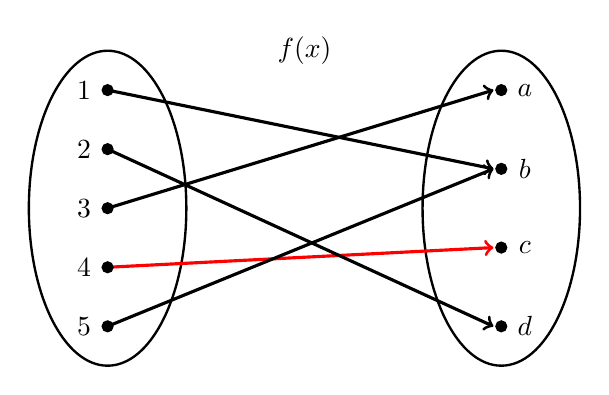
\begin{tikzpicture}
	\node at (2.5,2) {$f(x)$};
	% Ellipses
	\draw[line width=0.03cm] (0,0) circle (1 and 2);
	\draw[line width=0.03cm] (5,0) circle (1 and 2);
	
	\draw[line width= 0.04cm,->,red] (0,-0.75) -- (4.9,-0.5);
	
	% Nodes
	\draw[fill=black] (0,1.5) circle (0.07);
	\draw[fill=black] (0,0.75) circle (0.07);
	\draw[fill=black] (0,0) circle (0.07);
	\draw[fill=black] (0,-0.75) circle (0.07);
	\draw[fill=black] (0,-1.5) circle (0.07);
	
	\draw[fill=black] (5,1.5) circle (0.07);
	\draw[fill=black] (5,0.50) circle (0.07);
	\draw[fill=black] (5,-0.5) circle (0.07);
	\draw[fill=black] (5,-1.5) circle (0.07);
	
	
	% Arrow
	\draw[line width=0.04cm,->] (0,1.5) -- (4.9,0.50);
	\draw[line width=0.04cm,->] (0,0.75) -- (4.9,-1.5);
	\draw[line width=0.04cm,->] (0,0) -- (4.9,1.5);
	\draw[line width=0.04cm,->] (0,-1.5) -- (4.9,0.5);
	
	
	% Labels
	\node at (-0.3,1.5) {$1$};
	\node at (-0.3,0.75) {$2$};
	\node at (-0.3,0) {$3$};
	\node at (-0.3,-0.75) {$4$};
	\node at (-0.3,-1.5) {$5$};
	
	\node at (5.3,1.5) {$a$};
	\node at (5.3,0.5) {$b$};
	\node at (5.3,-0.5) {$c$};
	\node at (5.3,-1.5) {$d$};
	\end{tikzpicture}
	\]

\begin{enumerate}[(a)]
\item Explain why $f(x)$ is not a function. 
\item Add an arrow to the diagram so that $f(x)$ is a surjective function.
\item Identify the domain, codomain, and range for $f(x)$. 
\item Is $f(x)$ an injective function? Explain why or why not. 
\end{enumerate} \pspace

\sol 
\begin{enumerate}[(a)]
\item A function must be defined on its entire domain. Because the domain of $f(x)$ is the set $\{ 1, 2, 3, 4, 5 \}$, $f(4)$ need be defined for $f(x)$ to be a function. \pspace

\item For $f(x)$ to be a surjective function, we first need assure that $f(x)$ is a function, i.e. we need to define $f(4)$. We can choose any one of $\{ a, b, c, d \}$, i.e. $f(4) \in \{ a, b, c, d \}$. For $f(x)$ to be surjective, we need $\im f= \{ a, b, c, d \}$. As defined above, $\im f= \{ a, b, c, d \}$. But then defining $f(4)$ to be in $\{ a, b, c, d \} \setminus \im f= \{ c \}$, i.e. $f(4):= c$ (given by the red arrow in the diagram above), $f(x)$ is then a surjective function. \pspace

\item The domain of $f(x)$ is $\{ 1, 2, 3, 4, 5 \}$. The codomain of $f(x)$ is $\{ a, b, c, d \}$. The range of the original `function' was $\{ a, b, d \}$, while the range of the $f(x)$ defined is $\{ a, b, c, d \}$. \pspace

\item The function $f(x)$ is not injective as $f(1)= b= f(5)$ but $1 \neq 5$. 
\end{enumerate}



\newpage



% Problem 2
\problem{10} Complete the proof of the proposition stated below by filling in the blanks. \pspace

\noindent {\bfseries Proposition.} Let $f: X \to Y$ be a function and $B \subseteq Y$. Then $X \setminus f^{-1}(B) \subseteq f^{-1}(Y \setminus B)$. \pspace

\noindent {\itshape Proof.} We know that if $X \setminus f^{-1}(B)= \varnothing$, then $X \setminus f^{-1}(B) \subseteq f^{-1}(Y \setminus B)$. Assume that \pspace

$X \setminus f^{-1}(B)\neq \varnothing$. To show that $X \setminus f^{-1}(B) \subseteq f^{-1}(Y \setminus B)$, we need to show that if \uans{0.3cm}{$x \in X \setminus f^{-1}(B)$}, \pspace

then \uans{0.17cm}{$x \in f^{-1}(Y \setminus B)$}. \pvspace{0.7cm}

Let $x \in X \setminus f^{-1}(B)$. But then we know that \uans{0.95cm}{$x \in X$} and $x \notin$ \uans{0.85cm}{$f^{-1}(B)$}. Because \pspace

$x \notin$ \uans{0.85cm}{$f^{-1}(B)$}, we know that $f(x) \notin$ \uans{1.35cm}{$B$}. It is clear that $f(x) \in Y$. But then \pspace

\uans{0.72cm}{$f(x) \in Y$} and $f(x) \notin$ \uans{1.35cm}{$B$}. This shows that $f(x) \in$ \uans{1cm}{$Y \setminus B$}. \pspace

This shows that $f(x)$ is in the preimage of $Y \setminus B$. But then we know that $x \in$ \uans{0.55cm}{$f^{-1}(Y \setminus B)$}. \pspace

But then if $x \in$ \uans{0.53cm}{$X \setminus f^{-1}(B)$}, then $x \in$ \uans{0.55cm}{$f^{-1}(Y \setminus B)$}. Therefore, $X \setminus f^{-1}(B) \subseteq f^{-1}(Y \setminus B)$.



\newpage



% Problem 3
\problem{10} Let $f: \mathbb{R} \to \mathbb{R}$ be the function given by $x \mapsto x^2 + 3x - 7$. 
	\begin{enumerate}[(a)]
	\item Without referencing the graph of $f$, use the definition of decreasing to show that $f(x)$ is not a decreasing function on $\mathbb{R}$ by giving a counterexample. 
	\item Determine whether or not $3 \in \text{im } f$. If $3 \in \text{im } f$, find an element in the preimage of 3. If $3 \notin \text{im } f$, explain why. 
	\item Is $f^{-1}(x)$ a function? Explain why or why not by referencing the graph of $f(x)$. Give an additional explanation of why or why not using your response in (b). 
	\end{enumerate} \pspace

\sol 
\begin{enumerate}[(a)]
\item A function is decreasing if $f(x_2) \leq f(x_1)$ whenever $x_1 < x_2$. Observe that $0 < 1$ but $f(1)= -3 \not< -7= f(0)$. Therefore, $f(x)$ is not decreasing. [Note: We can write $f(x)= x^2 + 3x - 7= \left(x + \frac{3}{2} \right)^2 - \frac{37}{4}$. Therefore, $f(x)$ is decreasing on $(-\infty, -\frac{3}{2})$ and increasing on $(\frac{3}{2}, \infty)$.] \pspace

\item If $3 \in \im f$, then there exists $x_0 \in \mathbb{R}$ such that $f(x_0)= 3$. But then we would have\dots
	\[
	\begin{aligned}
	f(x_0)&= 3 \\[0.3cm]
	x_0^2 + 3x_0 - 7&= 3 \\[0.3cm]
	x_0^2 + 3x_0 -10&= 0 \\[0.3cm]
	(x_0 + 5)(x_0 - 2)&= 0 
	\end{aligned}
	\]
Then $x_0= -5$ or $x_0= 2$. One can easily verify that $f(-5)= f(2)= 3$. Therefore, $3 \in \im f$. \pspace

\item If $f^{-1}(x)$ is a function, then given $y \in \im f$, there is a unique $x$ such that $f(x)= y$. From (b), observe that given $3 \in \im f$, $f(-5)= f(2)= 3$. Therefore, $f^{-1}(3) \in \{ -5, 2 \}$ so that, as a function, $f^{-1}(3)$ is not well defined. Therefore, $f^{-1}(x)$ is not a function. 
\end{enumerate}


\end{document}